\chapter{Results \& Evaluation} \label{Results}

This chapter covers the evaluation of the developed payloads and defence mechanisms. 


\section{Payloads}

\section{Defence}

\subsection{Packet Analysis}

In the following, the captured packet will be analysed. The comparison is between the enumeration of an O.MG cable and two (TODO three?) unmodified external keyboards.   

In general, the devices' enumeration is very similar. They all follow the USB protocol correctly.  

\subsubsection{REMOTE WAKEUP}

Early in the enumeration, packet 16, the first big difference can be found: While all three external keyboards describe themselves to have the attribute 'REMOTE-WAKEUP' the O.MG cable specifies in the same packet that it has 'NO REMOTE WAKEUP'. This difference can be seen in figure \ref{fig:packet16OMG} vs \ref{fig:packet16Ducky}. 'REMOTE WAKEUP' means that the external keyboards have the function of sending a signal to a 'sleeping' host that can wake it. This is common for human interface devices and can, for example, be seen in mice that can be moved to wake a host. The cable, however, does not have that capability. When a payload is executed while the target is asleep, it is not woken up and therefore the input is not processed. For any of the external keyboards, any key can be pressed to wake the host. 

\begin{figure}[H]
    \centering
    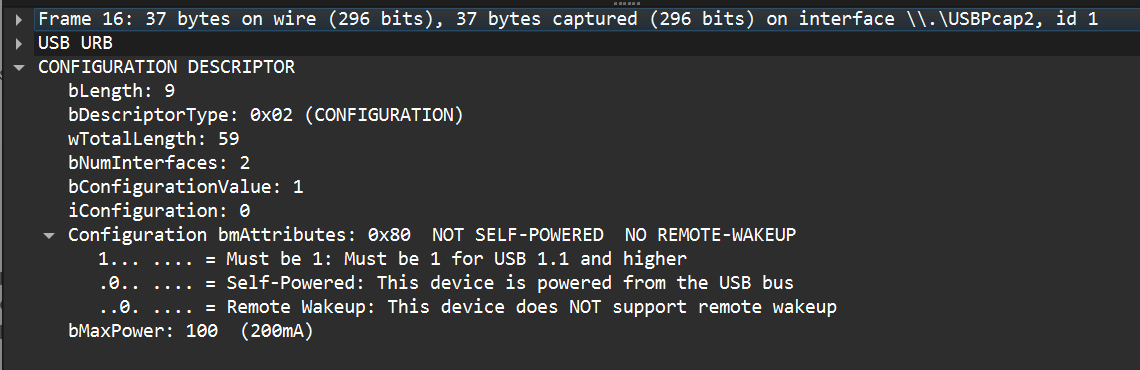
\includegraphics[width=0.75\linewidth]{visuals/no-remote-wakeup-100mA.png}
    \caption{Packet no. 16 of an O.MG Cable enumeration}
    \label{fig:packet16OMG}
\end{figure}

\subsection{Technical Data}

Just like the REMOTE WAKEUP property, the amount of power a non-self-powered device requires is specified within the first packets, specifically in packet nr 16. The difference that can be observed here is between the Ducky keyboard and the rest of the devices. While 3 of the 4 devices specify 'bMaxPower' in packet 15 to be "100 (200mA)" (figure \ref{fig:packet16OMG}, the Ducky's current consumption is "50 (100mA)" as seen in \ref{fig:packet16Ducky}. Maximum current consumption can therefore not be used as an indicator for the presence of an O.MG cable. 


\begin{figure}[H]
    \centering
    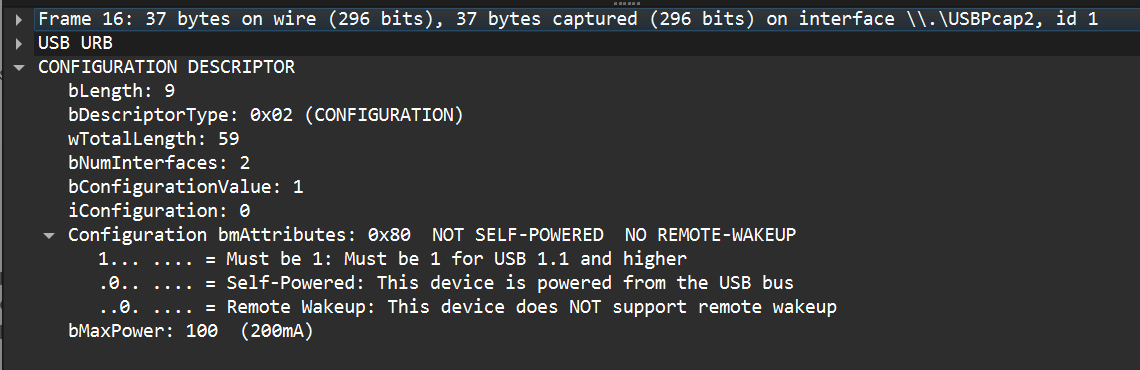
\includegraphics[width=0.75\linewidth]{visuals/no-remote-wakeup-100mA.png}
    \caption{Packet no. 16 of a Ducky Keyboard enumeration}
    \label{fig:packet16Ducky}
\end{figure}


\subsection{Register as multiple devices}

All the devices register as multiple HID devices. The Sharkoon and Glorious keyboards first register as a keyboard, then as a mouse. The Ducky registers as keyboard first and as multiple different 'HID Report's later. The O.MG cable is the only one that registers as a mouse first and as a keyboard second. This can be seen in packet 18 for all the devices; figure \ref{fig:packet18Glorious} shows an example of the Glorious Keyboard specifying the enumeration as keyboard and mouse. 


\begin{figure}[H]
    \centering
    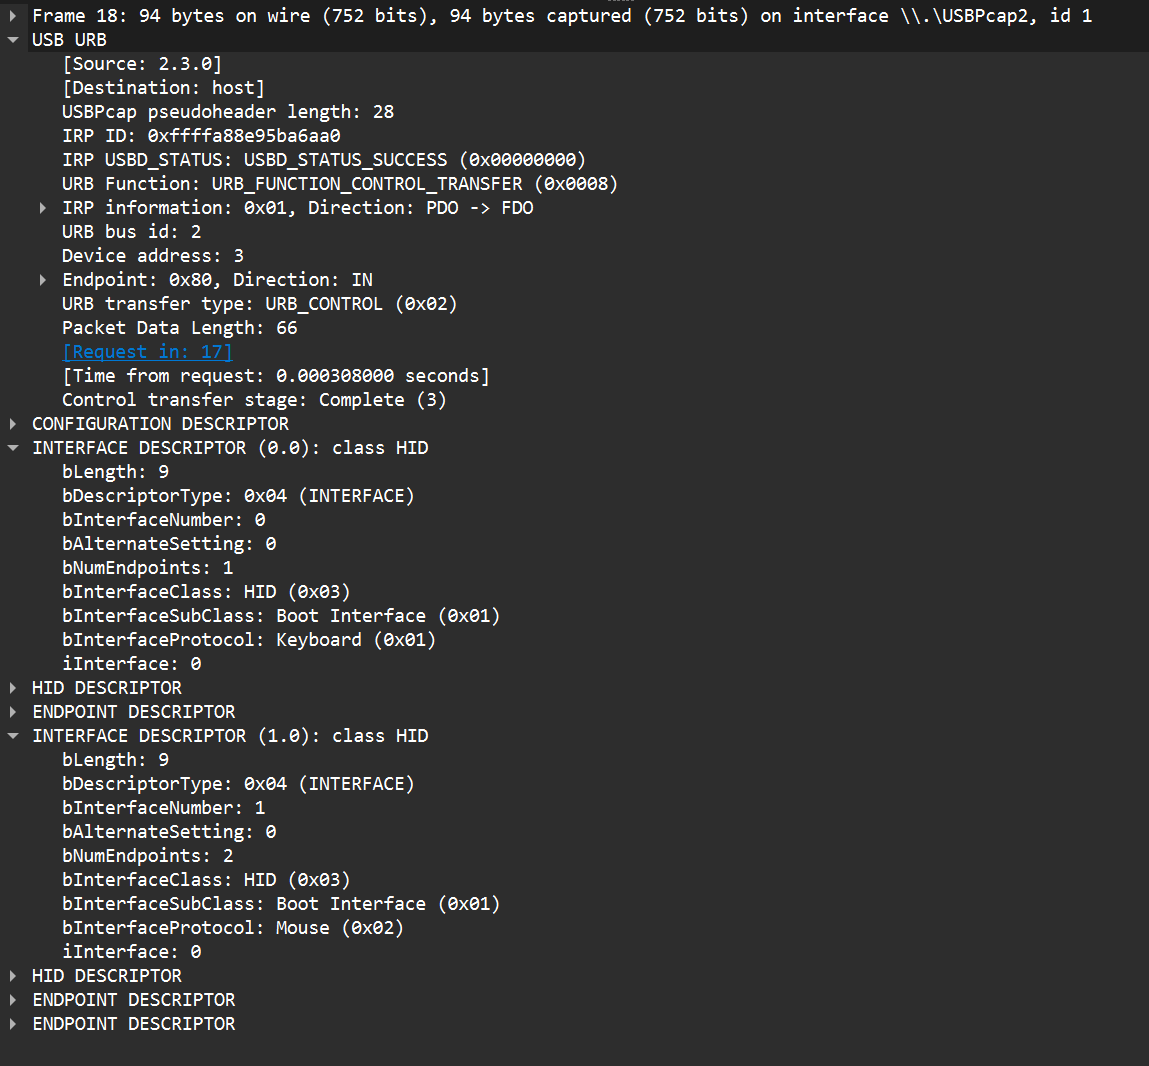
\includegraphics[width=0.75\linewidth]{visuals/packet18glorious.png}
    \caption{Packet no. 18 of a Glorious Keyboard enumeration}
    \label{fig:packet18Glorious}
\end{figure}

\subsection{Length of Descriptors}

In various instances the devices differ in their meta data. For example in packet 26 of the Sharkoon keyboard the bLength descriptor is 46, while for the Ducky it is 36, the Glorious 22 and the O.MG 10. Similarly, number for wLength differ in packet 27. These descriptors vary every time they occur, and between all the devices. Therefore, they cannot be used as a differentiator between malicious and harmless devices. Furthermore, since the lengths of the descriptors depend on the descriptors themselves, and the O.MG descriptors can easily be changed, this is not a reliable metric.
This also explains the differences in the bString itself, for example in packet 28, where the manufacturer's name is spelled out. Any manufacturer can easily be spoofed by an O.MG cable. 




\subsection{Unrecognized Packets}

All external keyboards have packet exchanges that Wireshark flags as 'Unknown type' which seems to be some Wireshark error for reading and interpreting the packets. The issue seems to have to do with the descriptors request that are specific for Windows \cite{USBPcapDidNot}. Noticeably, however, the O.MG does not have any 'Unknown type' packets in its enumeration.

\begin{figure}[H]
    \centering
    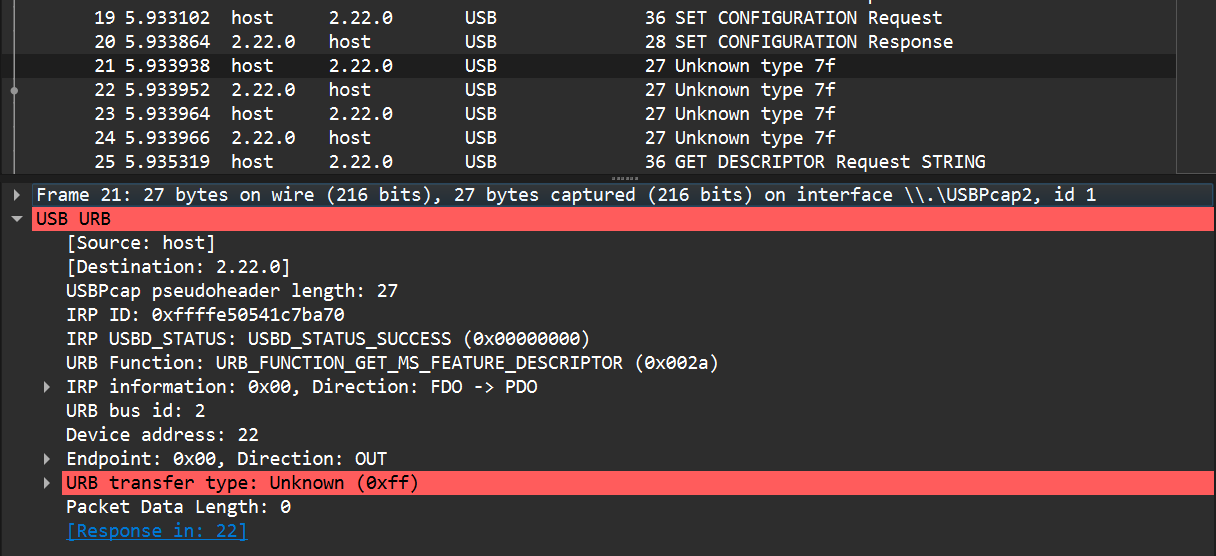
\includegraphics[width=0.75\linewidth]{visuals/unknownPacketsSharkoon.png}
    \caption{Unknown type Packets as an example from the Sharkoon enumeration}
    \label{fig:unknownPacketsSharkoon}
\end{figure}


\subsection{Larger Differences in Packet Types, Number and Order}

Due to some unrecognized packets and differences in enumeration order and the number and types of devices that are enumerated, the packets start to lose their alignment with each other around packet 30. From thereon, they are hard to compare directly. Some devices have more unrecognized packets, some different numbers of 'collection', 'usage page', 'usage', 'set\_report', and 'descriptor' packets. However, there seem to be no discernable patterns for this reason and the differences also occur within the harmless external keyboard group. From the sample size available, the O.MG has the smallest number of packets exchanged for enumeration. 


\subsection{Conclusion Packet Analysis}

The biggest difference in the enumeration phase of these devices is in the number and type of packets, however, they still follow the same pattern, given by the USB protocol. There does not seem to be a reliable pattern in this sample, however. A pattern might be found with a much bigger sample size and statistical analysis. This is out of scope for this thesis but should be considered in future works. (TODO; add this to limitations). Generally speaking, the cable seems to be more efficient than the external keyboards while enumerating using the least amount of packets overall.
Differences in descriptors, lengths and other meta data (like technical specifications) are non-conclusive for distinguishing the O.MG cable. 
The most apparent and striking difference is that the O.MG cable is enumerated with the 'NO REMOTE WAKEUP' attribute, which seems atypical for a HID device.
It is not surprising that the enumeration of the O.MG cable does not differ significantly from that of usual external keyboards. For the host, it looks like any other keyboard and functions like one too. Enumeration is therefore also the same. Additionally, the possible differences are restricted because of the established USB protocol.

It is important to note that while this thesis cannot conclude the presence of clear factors that point to the presence of an O.MG cable, it does not mean that they do not exist. Possibly patterns could be found with a scientific experiment featuring a big and statistically significant number of external keyboards (100+) and multiple O.MG cables.




